%% LaTeX2e class for student theses
%% thesis.tex
%% 
%% Karlsruhe Institute of Technology
%% Institute for Program Structures and Data Organization
%% Chair for Software Design and Quality (SDQ)
%%
%% Dr.-Ing. Erik Burger
%% burger@kit.edu
%%
%% See https://sdq.kastel.kit.edu/wiki/Dokumentvorlagen
%%
%% Version 1.3.6, 2022-09-28

%% Available page modes: oneside, twoside
%% Available languages: english, ngerman
%% Available modes: draft, final (see README)
\documentclass[oneside, english, draft]{sdqthesis}

%% ---------------------------------
%% | Information about the thesis  |
%% ---------------------------------

%% Name of the author
\author{Wenzhe Vincent Cui}

%% Title (and possibly subtitle) of the thesis
\title{Confidential Computing in Distributed Systems}

%% Type of the thesis 
\thesistype{Bachelor's Thesis}

%% Change the institute here, ``KASTEL'' is default
\myinstitute{SCC -- Steinbuch Centre for Computing}

%% You can put a logo in the ``logos'' directory and include it here
%% instead of the SDQ logo
% \grouplogo{myfile}
%% Alternatively, you can disable the group logo
% \nogrouplogo

%% The reviewers are the professors that grade your thesis
\reviewerone{Prof. A}
\reviewertwo{Prof. B}

%% The advisors are PhDs or Postdocs
\advisorone{M.Sc. C}
%% The second advisor can be omitted
\advisortwo{M.Sc. D}

%% Please enter the start end end time of your thesis
\editingtime{11. Month 2021}{02. Month 2022}

\settitle

%% --------------------------------
%% | Bibliography                 |
%% --------------------------------

%% Use biber instead of BibTeX, see README
\usepackage[citestyle=numeric,style=numeric,backend=biber]{biblatex}
\addbibresource{thesis.bib}

%% Todos
\usepackage[obeyDraft]{todonotes}

%% Tables
\usepackage{multirow}
\newcolumntype{L}[1]{>{\raggedright\arraybackslash}m{#1}}
\newcolumntype{C}[1]{>{\centering\arraybackslash}m{#1}}
\newcolumntype{R}[1]{>{\raggedleft\arraybackslash}m{#1}}

%% ====================================
%% ====================================
%% ||                                ||
%% || Beginning of the main document ||
%% ||                                ||
%% ====================================
%% ====================================
\begin{document}

%% Set PDF metadata
\setpdf

%% Set the title
\maketitle

%% The Preamble begins here
\frontmatter

%% LaTeX2e class for student theses: Declaration of independent work
%% sections/declaration.tex
%% 
%% Karlsruhe Institute of Technology
%% Institute for Program Structures and Data Organization
%% Chair for Software Design and Quality (SDQ)
%%
%% Dr.-Ing. Erik Burger
%% burger@kit.edu
%%
%% Version 1.3.6, 2022-09-28

\thispagestyle{empty}
\null\vfill
\noindent\hbox to \textwidth{\hrulefill} 
\iflanguage{english}{I declare that I have developed and written the enclosed
thesis completely by myself. I have submitted neither parts of nor the complete 
thesis as an examination elsewhere. I have not used any other than the aids that
I have mentioned. I have marked all parts of the thesis that I have included from 
referenced literature, either in their original wording or paraphrasing their
contents. This also applies to figures, sketches, images and similar depictions,
as well as sources from the internet.}%
{Ich versichere hiermit, dass ich die vorliegende Arbeit selbstständig verfasst,
und weder ganz oder in Teilen als Prüfungsleistung vorgelegt und keine anderen
als die angegebenen Hilfsmittel benutzt habe. Sämtliche Stellen der Arbeit, die
benutzten Werken im Wortlaut oder dem Sinn nach entnommen sind, habe ich durch
Quellenangaben kenntlich gemacht. Dies gilt auch für Zeichnungen, Skizzen,
bildliche Darstellungen und dergleichen sowie für Quellen aus dem Internet. }
 
 
%% ---------------------------------------------
%% | Replace PLACE and DATE with actual values |
%% ---------------------------------------------
\textbf{PLACE, DATE}
\vspace{1.5cm}
 
\dotfill\hspace*{8.0cm}\\
\hspace*{2cm}(\theauthor) 
\cleardoublepage

\setcounter{page}{1}
\pagenumbering{roman}

%% ----------------
%% |   Abstract   |
%% ----------------

\listoftodos
 
%% For theses written in English, an abstract both in English
%% and German is mandatory.
%%
%% For theses written in German, a German abstract is sufficient.
%%
%% The text is included from the following files:
%% - sections/abstract

%\includeabstract
%% LaTeX2e class for student theses
%% sections/abstract_en.tex
%% 
%% Karlsruhe Institute of Technology
%% Institute for Program Structures and Data Organization
%% Chair for Software Design and Quality (SDQ)
%%
%% Dr.-Ing. Erik Burger
%% burger@kit.edu
%%
%% Version 1.3.6, 2022-09-28

\Abstract

In the current computing landscape distributed computing systems, largely based
on Grid and Cloud computing, have become the main ways of sharing infrastructure
resources, such as compute, storage, and network resources, while also providing
services that ease the development and orchestration of applications on said
resources. On the one hand, the usage of these resources and service come with
benefits such as higher availability, reducing complexity of applications, and
cost-efficiency, on the other hand, traditionally these benefits come with the
cost of fully trusting the provider of the resources and services with
potentially confidential data. Nevertheless, as consumer and government demands
for data privacy increase (e.g., GDPR coming into effect in the EU in 2018), the
distributed computing model must adapt to meet the increasingly strict trust
requirements. The advent of confidential computing enables a new distributed
computing model where the provider of infrastructure resources becomes untrusted
by providing hardware-based trusted execution environments (TEEs). This thesis
researches the current state of trusted execution environment technologies,
remote attestation procedures that allow tenants to verify the trustworthiness
of TEEs, and introduces a new \textit{trusted distributed computing model} that
integrates these two concepts into the traditional distributed computing model
in order to remove the provider of the distributed computing system from the
list of trusted parties.


%% ------------------------
%% |   Table of Contents  |
%% ------------------------
\tableofcontents

\listoffigures
\listoftables

%% -----------------
%% |   Main part   |
%% -----------------

\mainmatter

\chapter{Introduction}
\label{ch:Introduction}

%% LaTeX2e class for student theses
%% sections/content.tex
%% 
%% Karlsruhe Institute of Technology
%% Institute for Program Structures and Data Organization
%% Chair for Software Design and Quality (SDQ)
%%
%% Dr.-Ing. Erik Burger
%% burger@kit.edu
%%
%% Version 1.3.6, 2022-09-28

\chapter{Introduction}
\label{ch:Introduction}

\section{Background}
\label{sec:background}

\section{Motivation}
\label{sec:motivation}

\section{Research Methodology}
\label{sec:research-methodology}


\chapter{Terminology}

\chapter{Terminology}

\section{Terms}

\subsection{Platform}

Group of technologies and services that are used as a base upon which
applications are developed and deployed.

\todo[inline]{Expand explanation of term `Platform'}
\todo[inline]{Go more into dynamic infrastructure management}

\subsection{Confidentiality}
\label{sec:confidentiality}

Isolation techniques like containerization and virtualization protect the
infrastructure or platform from applications. On the other hand confidentiality
is the direct opposite and its goal is to protect the application from the
infrastructure or platform it is running on.

\subsection{Trusted Computing Base (TCB)}

The set of all hardware, firmware, and/or software components that are critical
to the security of a given computing system. These components are the only
components in the computing system that operate at a high level of trust. This
does not imply that these components are secure, but that they are crucial to the
security of system as a whole.

\section{Roles}

While this section defines roles and their tasks, one should keep in mind that a
single entity can take on multiple roles. Section \ref{sec:trust-model} will
define which roles shouldn't be aggregated onto one entity.

\todo[inline]{Remove term ``client'' from document}

\subsection*{Infrastructure Provider}

The infrastructure provider controls the hardware and firmware used to provide
compute, networking, and storage resources.

\subsection*{Service Provider}

An entity providing services on top of infrastructure provided by the
infrastructure provider in order to ease the development and deployment of
applications -- often in the form of a platform.

\subsection*{Application Owner}

An entity developing an application for a customer on the platform provided by
the service provider.

\subsection*{Data Owner}

An entity that is in the possession of possibly sensible data that will be
processed or used by an application deployed on the platform provided by the
service provider.

\subsection*{Verifier}

An entity that verifies that the services provided by the service provider can
be trusted.


\chapter{Background}

\section{Virtualization}

\subsection{Virtual Machine Manager (VMM)}

\section{Containerization}

\begin{figure}
  \centering
  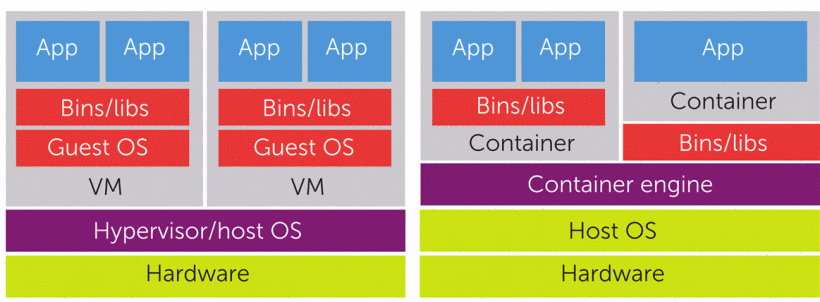
\includegraphics{resources/vm-vs-container.png}
  \caption{
    A comparison between VM and container based virtualization architectures\\
    Source: \citetitle{ieee-containers} \cite{ieee-containers}
  }
  \label{fig:vm-vs-container}
\end{figure}

For a long time VMs have been the standard virtualization technology used in
cloud environments in order to provide virtualized infrastructure with an
abstraction level at the operating system level. While containers are also a
virtualization technique, VMs and containers address different problems. VMs
allow virtual hardware allocation and management, while containers address the
issue of interoperable applications. In the cloud environment (see chapter
\ref{sec:cloud-computing}) VMs focus on the infrastructure layer while
containers are used in the platform layer \cite{ieee-containers}.

While VMs have been used in order to schedule processes as manageable units they
require a file system containing a full operating system. This results in large
memory and storage requirements and slow startup times. In contrast, containers
share their OS with the host they are running on and only hold application code,
runtime, system tools, and system libraries needed for the application (see
figure \ref{fig:vm-vs-container}). This enables interoperability while making
containers lightweight.

Today most containerization technologies are based on the Linux Container (LXC)
technique. LXC facilitates namespace isolation, which allows groups of processes
to be separated. This prevents the (read and write) access to other resources
running on the same host and is used to isolate processes, inter-process
communication, networking, mount points, and kernel and version identifiers.

A container describes a running instance of a container image. While VMs mount
the file root file system in read-write mode (after executing integrity checks),
containers mount the root file system as read-only and utilize union mounts in
order to add a writable file system on top of the read-only root file system.
This allows easier distribution and replacement of images, even for existing
containers.

\subsection{Container Runtime (CR) and Container Manager (CM)}
\label{sec:container-runtime}

\todo[inline]{Use OCI specifications to make this section clearer}
\todo[inline]{Explain container image registry}

Container runtimes are the pieces of software that manage the lifecycle of
containers. Today these runtimes fall mostly fall into two categories, low-level
and high-level runtime. While low-level runtimes like runc or kata are only
responsible for spawning and running containers on the host, high-level runtimes
like containerd or cri-o build on top of low-level runtimes and also manage
container images. In order to differentiate and avoid confusion we will refer to
high-level runtimes as container managers in this thesis.


\chapter{Technical Research}

\section{Distributed Resource Management Systems}
\label{sec:distributed-resource-management-systems}

Examples
\begin{itemize}
  \item Grid
  \item Cloud
\end{itemize}

\subsection{Definition}

\citetitle{mell2011} \cite{mell2011} defines cloud computing as a model in order
to enable ``ubiquitous, convenient, on-demand network access to a shared pool of
configurable computing resources [...] that can be rapidly provisioned and
released with minimal management effort or service provider interaction''. It
extracts essential characteristics, service models, and deployment models:

\subsubsection{Characteristics}

\begin{itemize}
  \item On-demand self-service
  \item Broad network access
  \item Resource pooling
  \item Rapid elasticity
  \item Measured service
\end{itemize}

\subsubsection{Service Models}

\begin{itemize}
  \item Software as a Service (SaaS)
  \item Platform as a Service (PaaS)
  \item Infrastructure as a Service (IaaS)
\end{itemize}

\subsubsection{Deployment Models}

\begin{itemize}
  \item Private cloud
  \item Community cloud
  \item Public cloud
  \item Hybrid
\end{itemize}

\section{Confidential Computing}
\label{sec:confidential-computing}

Moving on from the traditional distributed computing model, this section gives
an overview of the current state of confidential computing.

Data can be in three distinct states: ``at rest'', ``in transit'', and ``in
use''. These three states describe data stored in persistent storage, traversing
a network, and data currently being processed by an application. While
technologies protecting data at rest and in transit are commonly used today,
there are not many methods to protect data in use.

Confidential computing provides hardware-based primitives that allow the
creation of trusted execution environments (TEEs). These TEEs have specific
properties that protect data in use.

\subsection{Trusted Execution Environments (TEEs)}
\label{sec:tee}

\subsubsection{Properties}

There are different definitions of a trusted execution environment (TEE) with
varying properties. The three main properties defined by the
\textit{Confidential Computing Consortium} \cite{ccc2022technicalanalysis} are:

\begin{description}
  \item[Data confidentiality]
    Prevent unauthorized entities from viewing data that is in use within a TEE.
  \item[Data integrity]
    Prevent unauthorized entities from adding, removing, or changing data while
    it is in use within a TEE.
  \item[Code integrity]
    Prevent unauthorized entities from adding, removing, or changing code
    executed in the TEE.
\end{description}

Besides ensuring the confidentiality of data, code integrity is also critical
for the confidentiality of data. Even if data confidentiality is implemented
correctly, executing compromised code inside TEEs can also lead to confidential
data leakage.

Provided that the application code implements the computation correctly, data
and code integrity ensure that neither the data nor the application has been
modified, allowing clients to trust the results of the computations run inside
TEEs.

As TEE technologies widely differ in their implementations, this thesis will
treat the hardware and software components that create and protect TEEs as a
single platform consisting of all hardware and software components involved, and
refer to it as the ``TEE platform''.

Besides the three core properties, TEE platforms also often provide mechanisms
that enable the integration of a remote attestation process (see Section
\ref{sec:remote-attestation}), enabling clients to assess the trustworthiness of
TEEs created by an untrusted party. These technologies generally produce
evidence about the authenticity and integrity of both the TEE platform and
specific TEEs.

\subsubsection{Hardware Support}

The security of a software layer can only be as strong as the layers below it.
This is why an ideal security solution acts from the lowest layer possible. By
providing security through the lowest layer -- the hardware -- it is possible to
remove almost all software components between the hardware and the TEE from the
list of trusted components, including system software such as the operating
systems and hypervisors. The only components that need to be trusted are the
components of the TEE platform.

Today most TEE implementations still rely on firmware components that are part
of the TEE platform, allows manufacturers to deploy bug fixes and security
patches. Because an untrusted service provider can compromise these firmware
components, TEE platforms generally facilitate hardware-based mechanisms that
produce evidence about the integrity of the TEE platform.

\subsubsection{Memory Protection}

Most TEE technologies today rely on the protection of memory to provide the
three properties defined above. They often implement two mechanisms, protecting
the confidentiality and integrity of data stored in memory:

\begin{description}
  \item[Memory Encryption]
    TEE technologies rely on hardware components to encrypt data that is being
    transferred from the CPU to the physical memory of a machine and decrypt
    data moving from the memory to the CPU. Unlike homomorphic encryption, which
    provides specific computational functions directly on encrypted data
    \cite{monique2013homomorphicencryption}, TEE technologies transparently
    en-/decrypt data. Most importantly, the unencrypted data is only available
    while being processed by the CPU, and is encrypted before leaving the CPU.
    Memory encryption strengthens the confidentiality of data in use, as
    untrusted software components that gain access to the memory of a TEE or
    malicious entities that have physical access to the machine only see
    encrypted data.

  \item[Memory Access Control]
    On the other hand, memory integrity is guaranteed by enforcing that only the
    TEE owning a specific memory region can modify data stored in this region.
    In order to achieve this, the TEE platform has to keep track of protected
    memory pages, and their owners.
\end{description}

\subsection{TEE Models}
\label{sec:tee-models}

There are two distinct models of TEEs, process-based and VM-based.

\subsubsection{Process-based TEEs}
\label{sec:process-based-tees}

Process-based TEEs introduce a new programming model. A program needs to be
split into two components, trusted and untrusted. These are often referred to as
the ``enclave'' and ``host''. The enclave is executed in a TEE and, as such,
should contain all code that interacts with confidential data, whereas the host
component is responsible for handling non-sensitive tasks like networking and
file I/O.

While the host is not shielded, the enclave is protected from the rest of the
system, including:

\begin{itemize}
  \item the enclave's own host
  \item other processes running on the same machine
  \item the operating system
  \item firmware such as the BIOS
  \item the hypervisor and host operating system (in virtualized environments)
  \item hardware other than the processor
\end{itemize}

Splitting a program into enclave and host is challenging. It requires a deep
understanding of security and how these process-based TEE solutions work. SDKs
and frameworks often hide the split between host and enclave from developers to
ease the development of such applications \cite{schuster2022}.

Library OSes like Gramine and Occlum go even further and provide a POSIX-like
runtime environment with network, file I/O, and multithreading support. Because
applications running inside the enclave do not have access to the underlying OS,
library OSes provide libraries that implement OS system calls in the form of
library functions, while a boilerplate host provides I/O functionalities
\cite{tsai2014graphene}.

Even though these SDKs, frameworks, and library OSes ease the development, using
process-based TEEs still requires more development effort, and porting existing
applications often still requires the modification of the application.

\subsubsection{VM-based TEEs}
\label{sec:vm-based-tees}

The central concept of VM-based TEEs is to apply the TEE properties to a whole
virtual machine. Traditionally, hypervisors are fully responsible for managing
VM memory and thus have access to VM memory. On the other hand, TEE platforms
offering VM-based TEEs take away the responsibility of VM memory protection from
the hypervisor because the TEE platform itself already implements memory
protection. So instead of having full access to a VM's memory, the hypervisor
now only manages VM memory through mechanisms offered by the TEE platform.

VM-based TEEs are specifically designed to protect VMs from the rest of the
system, including:

\begin{itemize}
  \item VM firmware (e.g., OVMF)
  \item the hypervisor and/or host operating system
  \item hardware other than the processor
\end{itemize}

\subsubsection{Comparison}

Figure \ref{figure:cc-tee-comparison} compares the list of trusted components of
an application running without confidential computing, inside a process-based
TEE, and inside a VM-based TEE. In both TEE models the TEE platform enforces the
TEE properties and thus the hardware has to be partly trusted. 

On the one hand, process-based TEEs allow fine-grained separation of trust by
splitting applications into host and enclave, but this requires applications to
be ported to a new programming model. On the other hand, VM-based TEEs have much
larger attack surfaces because they include an entire OS but allow complex
applications to be run in a more secure environment without the need to modify
the applications.

\begin{figure}[H]
  \centering
  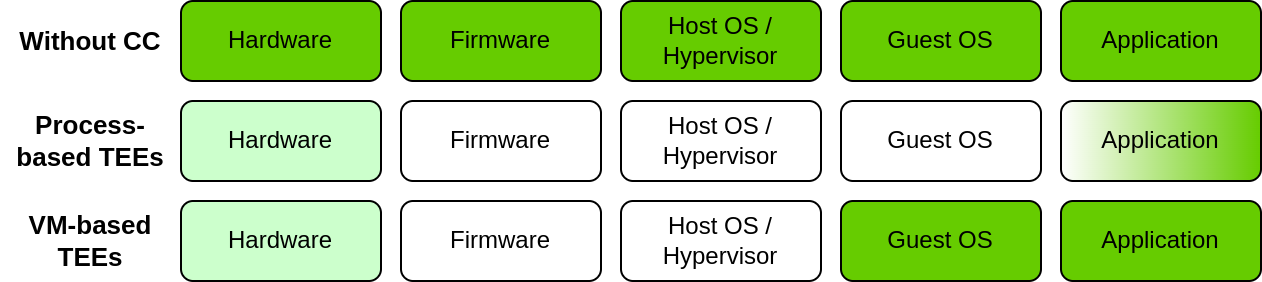
\includegraphics[width=0.85\linewidth]{resources/tee-models-comparison.drawio.png}
  \caption[Comparison of TEE models.]{
    Comparison of TEE models. In both TEE, cases the hardware has to be partly
    trusted, illustrated by the lightly marked hardware components. In the
    process-based TEE model, the application has to be split into enclave and
    host, which is why the application component is marked with a gradient.
  }
  \label{figure:cc-tee-comparison}
\end{figure}

\subsection{Commercially Available TEE Technologies}
\label{sec:commercial-tee-technologies}

\begin{description}
  \item[Intel SGX]
    Intel Software Guard Extensions (SGX) provides process-based TEEs by relying
    on hardware to create enclaves that contain application code and
    confidential data. As the name implies, it is an extension of Intel's CPU
    instruction set architecture \cite{costan2016sgx}.

    The CPU protects a designated memory area called the Processor Reserved
    Memory (PRM) established by SGX by ensuring that other software and hardware
    components, such as system software (hypervisor or OS) and DMA devices, do
    not have access to the PRM. Confidential data and enclave application code
    is stored in the Enclave Page Cache (EPC), a subset of the PRM. SGX relies
    on untrusted system software to manage EPC pages by assigning EPC pages to
    enclaves and evicting these pages if needed. However, system software cannot
    directly access the EPC, and the CPU maintains Enclave Page Cache Map (EPCM)
    in the EPC that keeps track of allocated EPC pages and the enclave which
    owns the page. Using the EPCM, the CPU checks the correctness of the system
    software's allocation decisions, ensures that an EPC page is only assigned
    to a single enclave, and that only the assigned enclave can access and
    modify the EPC page. The CPU also encrypts EPC pages while they are stored
    in physical memory to prevent leaking confidential data through PME attacks
    and guarantee the confidentiality of data stored in EPC pages after
    eviction.

    Initially, the system software asks the CPU to copy data from unprotected
    memory into EPC pages and assigns the pages to the enclave. After the EPC
    pages are loaded, the enclave is marked as initialized, and the system
    software can not access nor modify EPC pages anymore. The CPU then measures
    SGX firmware components and the EPC pages of the enclave, producing
    attestation evidence which is then signed by the CPU using a cryptographic
    key that is only accessible by the CPU. The signature can then be used to
    verify the authenticity of the evidence, which in turn can be used to verify
    the integrity of the enclave and the SGX platform. An attestation can not
    only be requested after initialization but also during runtime.

  \item[AMD SEV]
    AMD SEV-SNP is the latest iteration of AMD's Secure Encrypted Virtualization
    (SEV) technology \cite{amd2021sev, amd2017seves, amd2020sevsnp} and, as the
    name implies, provides VM-based TEEs.

    SEV relies on hardware-embedded encryption engines that encrypt or decrypt
    memory pages written to or read from the physical memory of a machine. It
    utilizes the AMD Secure Processor (AMD-SP), which is integrated into the
    same chip as the CPU, to generate and manage cryptographic keys used for the
    en-/decryption. All software and data are tagged with an Address Space
    Identifier (ASID). The CPU uses the ASID to restrict data access and
    modification to the owner with the same ASID, protecting data from any
    unauthorized usage. However, in the first iteration of SEV, the registers of
    a virtual CPU could be used to leak confidential data when shutting down a
    VM. Subsequently, AMD released their second iteration SEV-ES (Encrypted
    State), which encrypts VM memory and virtual CPU registers. The latest
    version SEV-SNP (Secure Nested Paging), introduced additional features that
    protect VM memory integrity.

    The attestation process for SEV VMs is similar to the attestation process
    for SGX enclaves. A hypervisor launches a VM, and after the VM is fully
    loaded, the VM's memory is encrypted. Subsequently, the AMD-SP measures SEV
    firmware components and VM memory pages, which are signed using a
    cryptographic key only accessible by the CPU. Again, the signature can then
    be used for verifying the authenticity of the measurements, and the
    measurements can be used for verifying the integrity of the VM and the SEV
    platform. Attestation support in SEV and SEV-ES was limited, as measurements
    could only be requested during the launch of a VM. SEV-SNP supports the
    request for measurements at any time, enabling a more flexible remote
    attestation.
\end{description}

\subsection{Limitations}
\label{sec:limitations}

\begin{description}
  \item[Performance Impact]
    Existing solutions require careful configuration to achieve acceptable
    performance or are inappropriate for specific use cases
    \cite{akram2021performance}. For example, due to the limited size of the EPC
    and the restricted programming model, Intel SGX displays a significant
    performance loss for high performance workloads, making the usage of SGX for
    these kinds of cases impractical.
  \item[CPU centric focus]
    Most of today's confidential computing solutions focus on a CPU-level view
    of memory permissions. This limits the application of confidential computing
    to heterogeneous computing systems, where discrete accelerators are used in
    order to speed up specific computations (e.g. GPUs and NPUs for machine
    learning workloads). However, there is ongoing work on integrating
    confidential computing into heterogeneous computing systems
    \cite{jiang2022cronus}.
  \item[New technology that requires further research]
    Since the introduction of Intel SGX in 2015, numerous vulnerabilities have
    been found in the SGX architecture \cite{fei2021sgxvulnerabilities}. AMD SEV
    has also not been spared, which until now required two iterations to fix the
    issues that have been discovered. Both technologies also depend on existing
    software, such as operating systems, hypervisors, and VM firmware, to
    implement the support of these technologies. These implementations also
    require further research and testing to find vulnerabilities and security
    issues.
\end{description}

\section{Remote Attestation}
\label{ch:remote-attestation}

Running applications inside a CC enabled environment is not enough in order to
deepen the trust with the client or third-parties. In order to prove that the
application is running inside a CC enabled environment and that neither the
application nor the system it is running on has been tampered with, the provider
can employ remote attestation.

In a remote attestation environment there are at least two roles: the attester
and the relying party. The attester produces information about itself
(evidence), on which the relying party makes a decision whether to trust the
attester or not.

In our context the attester would be the system running a client application and
the relying party would be the data owner.

\subsection{Remote Attestation Procedures (RATS)}
\label{sec:rats}

\begin{figure}
  \centering
  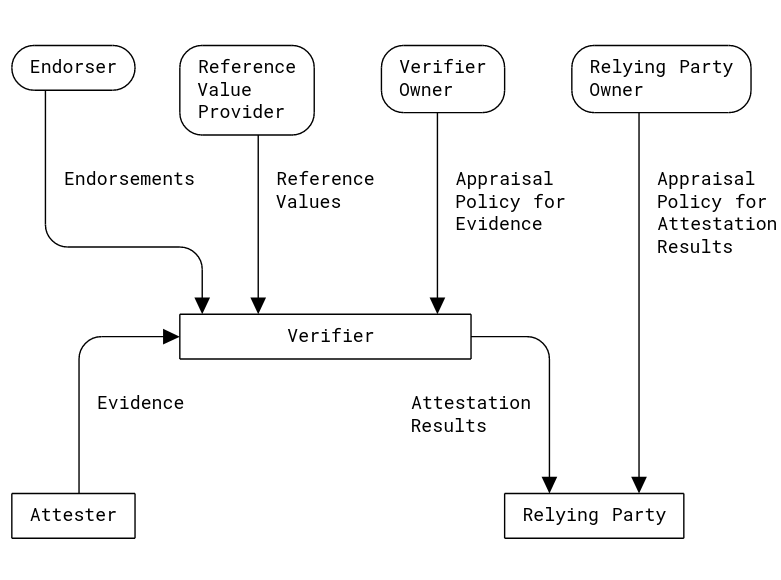
\includegraphics[width=0.7\linewidth]{resources/rats-architecture.png}
  \caption[RATS architectural overview]{
    RATS architectural overview.\\
    Source: \citetitle{rfc9334} \cite{rfc9334}
  }
  \label{figure:rats-architecture}
\end{figure}

Remote Attestation Procedures (RATS) defines a general architecture, roles, and
messages in order to establish trust between the relying party and the attester.
Figure \ref{figure:rats-architecture} shows the general architecture. RATS
introduces few new roles where the most prominent one is the verifier. It
produces attestation results by using evidence, endorsements, reference values,
and applying an appraisal policy to assess the trustworthiness of the attester.
These attestation results then support the decision process of the relying party
on whether to trust the attester or not. We will go into more detail in chapter
\ref{sec:proposal:architecture}.

\section{Existing Solutions}

\subsection{Commercial Solutions by well-known Service Providers}

\begin{description}
  \item[AWS Nitro]
    \todo[inline]{Description: AWS Nitro}
    \begin{itemize}
      \item More of a TEE technology
      \item Doesn't solve trust problem with the service provider
    \end{itemize}
  \item[Confidential VMs (Azure, GCP)]
    \todo[inline]{Description: Azure Confidential Containers}
    \begin{itemize}
      \item AMD SEV enabled VMs or VMs providing Intel SGX capabilities
      \item Verification has to be implemented by the customer
    \end{itemize}
  \item[GCP Confidential Dataproc]
    Big data processing through fully managed data processing frameworks and
    tools like Spark and Hadoop. Uses confidential VMs to provide
    confidentiality.
    \todo[inline]{Dataproc: Verification of nodes?}
  \item[GCP Confidential Space]
    Let multiple parties share confidential data with a workload while retaining
    the confidentiality and ownership of the data.
    \todo[inline]{Confidential Space: More research needed}
\end{description}

\todo[inline]{Problems with commercial solutions}

\subsection{Kubernetes as platform base}

Kubernetes is an extensible, open source platform for managing containerized
workloads and services. Due to its open source nature and popularity there has
been a rapidly growing ecosystem surrounding Kubernetes. It provides general
platform features such as deployment, orchestration, scaling, load-balancing,
integration with logging, monitoring, and alerting solutions.

A simplified overview over core components inside a Kubernetes cluster (see
figure \ref{fig:kubernetes-overview}):

\begin{figure}
  \centering
  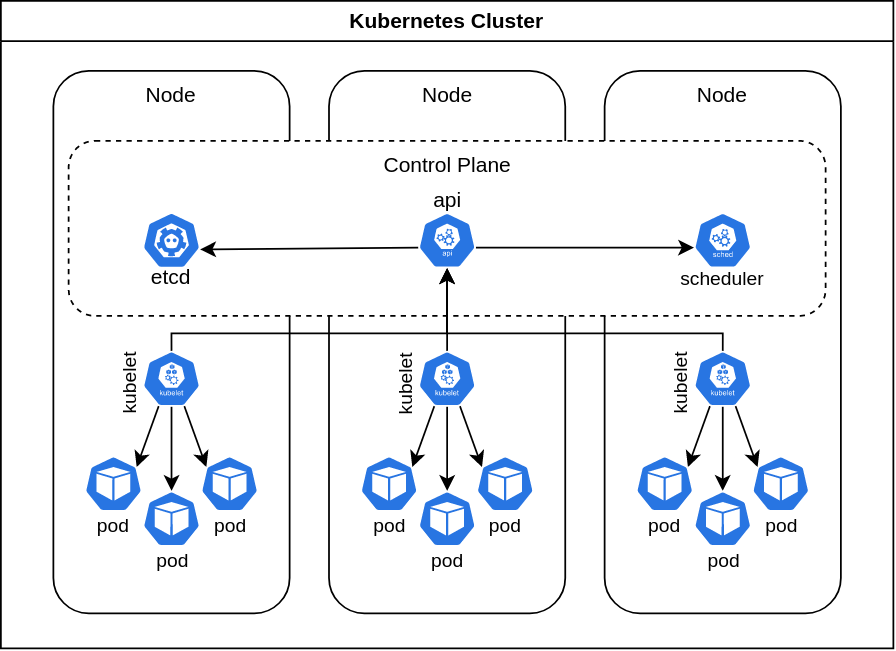
\includegraphics[width=0.8\linewidth]{resources/kubernetes-overview.png}
  \caption{A simplified overview over the Kubernetes components.}
  \label{fig:kubernetes-overview}
\end{figure}

\begin{description}
  \item[Nodes]
    (Possibly virtual) machines running containerized applications. On each node
    runs a component called kubelet that manages the pods and the corresponding
    containers on the node.
  \item[Pods]
    A group of containers that share storage and network resources that models
    an application-specific logical host. The containers that make up a pod are
    always located on the same node and are scheduled in unison.
  \item[Control Plane]
    A collection of pods that manage the nodes and workload pods inside the
    cluster. This includes an API, a backing store (etcd) for all cluster data,
    and a scheduler that assigns pods to nodes.
  \item[Container Runtime]
    Responsible for executing containers on a node (see section
    \ref{sec:container-runtime}).
\end{description}

\todo[inline]{Kubernetes: Expand as needed in the next chapters}

Kubernetes' non-monolithic design allows the replacement of almost every aspect
and component of a cluster. This allows a Kubernetes cluster to be run on
basically any underlying infrastructure, regardless of the hardware choices or
networking design.

There are three levels in a Kubernetes cluster on which confidentiality can be
applied to: The node, pod, or container. There are distinct benefits and
problems for applying confidentiality on each layer. We will discuss them in the
following sections.

\subsubsection{Confidential Nodes}

The most outer layer where confidentiality can be applied to in the Kubernetes
architecture are the nodes. By using confidential computing enabled virtual
machines -- for example by facilitating AMD SEV or Intel TDX -- a Kubernetes
cluster operator is able to shield workloads running inside the cluster.
Prominent service providers like Azure and GCP already offer the option of
deploying their managed Kubernetes clusters with confidential worker nodes.
However, these solutions don't include verification of the nodes which means
that one would have to build a custom remote attestation system -- for example
by implementing the RATS (section \ref{sec:rats}).

The biggest problem with confidential nodes is the restriction of cluster admin
privileges and verifying these as a client. While the workloads are shielded
from the infrastructure cluster administrators would still have full control
over the workloads running inside the cluster which breaks goal
\subGoalRef{2}{1}.

\subsubsection{Confidential Containers}

The other extreme would be to apply confidentiality to containers. A process
running inside a TEE would only receive confidential data like decryption keys
or personalized information after verifying that the process is running inside a
TEE via remote attestation. Since the TEE shields the process from the cluster
this approach remove the cluster administrator from the TCB of the application.

Even though this approach doesn't conflict with the goals of this paper, it does
collide with the design of Kubernetes. In the Kubernetes architecture the
smallest deployable unit of computation is a pod, a collection of application
containers. These containers share storage and network resources, but it becomes
very hard to share these resources when the containers are shielded from each
other. The next approach addresses this architectural issue.

\subsubsection{Confidential Pods}
\label{sec:confidential-applications}

Instead of applying confidentiality to containers we can also shield pods from
the outside world. This improves the last approach as per definition a pod in a
Kubernetes cluster defines an application-specific logical host. As opposed to
shielding a single container, shielding a pod would allow sharing storage and
networking resources between containers composing the pod.


% Main Content

\chapter{Traditional Platform Architecture}

\todo[inline]{Generalized traditional platform architecture}

%% LaTeX2e class for student theses
%% sections/proposal.tex
%% 
%% Karlsruhe Institute of Technology
%% Institute for Program Structures and Data Organization
%% Chair for Software Design and Quality (SDQ)
%%
%% Dr.-Ing. Erik Burger
%% burger@kit.edu
%%
%% Version 1.3.6, 2022-09-28

\chapter{Secure Computation Platform Proposal}
\label{ch:proposal}

\section{Trust Model}
\label{sec:trust-model}

In the following chapter we will often refer to entities and components as
``trusted'' and ``untrusted''. This trust relation is defined from the
perspective of the data owner as this role is in possession of the sensitive
data.

\subsection{Roles}

\subsubsection{Infrastructure and Service Provider}

The infrastructure provider is responsible for the availability of the
infrastructure used to provide compute, networking, and storage resources. As
such the infrastructure controls and has access to the physical hardware and
firmware.

On the other hand the service provider is responsible for managing services that
utilize the infrastructure provided by the infrastructure provider in order to
ease the development and deployment of workloads. As such the service provider
is not only responsible for deploying the applications, but also to provide
services that allow the retrieval of attestation evidence and initialize TEE
environments.

As stated in the introduction the goal is to remove these two entities from the
trust model of the application. For this reason both roles can be aggregated in
the same entity.

\subsubsection{Application Owner}

The application owner designs and implements application workloads that will be
deployed and orchestrated by the service provider. This role needs to prove to
the customer aspects of compliance to the defined requirements. It also defines
computing resource requirements for the application workloads in order to run
and maintain compliance.

\subsubsection{Data Owner}

As the owner of the confidential data, this role is concerned with the
visibility and integrity of their data and the compliance of the application
with the requested requirements.

\subsubsection{Verifier}

In order to remove the service provider from the application's trust model, an
external party has to verify the service provider's confidentiality claims. The
verifier provides an attestation service that appraises evidence and returns
attestation results.

\section{Architecture}
\label{sec:proposal:architecture}

\subsection{Overview}

\begin{figure}
  \centering
  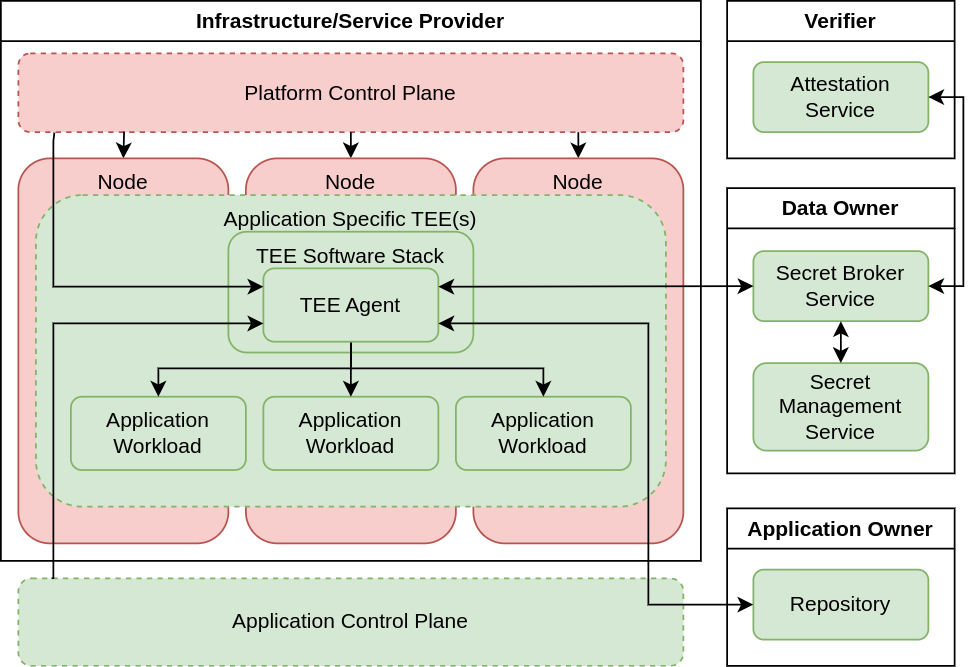
\includegraphics[width=\linewidth]{resources/architecture-overview.png}
  \caption[A simplified overview over the Confidential Containers architecture]{
    An overview over components used in this architecture proposal. Defines
    which components are managed by which role and whether it is trusted.
    Entities and Components marked in red are untrusted, while those marked in
    green are trusted.}
  \label{fig:proposal:architecture-overview}
\end{figure}

For convenience, from now on we will refer to confidential data as ``secrets''.
Figure \ref{fig:proposal:architecture-overview} shows an overview over the
components used in this architecture proposal, aiding the reader with
understanding the relation between the components introduced in the next
section.

\subsection{Components}

\subsubsection{Control Planes}

In a dynamically provisioned platform managing the infrastructure and
orchestrating applications is the responsibility of the control plane. We are
grossly simplifying the control plane here by considering it as a single
component. In traditional platforms the control plane is a high-privileged
component in order to perform management and orchestration tasks.

We want to apply the least privileges principle to the control plane and only
allow privileges necessary for basic management and orchestration. This includes
managing the lifecycle of applications on a node, migration of applications
between nodes, and monitor computing resource usage. But privileges that have
the potential to compromise the integrity of application code and data should
only be assigned to trusted entities and components. This implies that entities
and components controlled by the service provider should not have these
privileges.

To achieve this the traditional control plane has to be split into a platform
and an application control plane. As stated above the platform control plane
manages and orchestrates the platform with only the set of permissions that is
needed to achieve this. On the other hand the application control plane is
responsible for everything that directly interacts with the application. To make
the split of the control plane effective the service provider can not control or
have access to the application control plane. This implies that an external
entity like the application or data owner has to manage this control plane
instance.

\subsubsection{TEE Agent}

TEEs are designed to shield everything within the environment from the outside.
Because the control plane is not part of a specific application TEE, the control
plane is not able to interact with applications inside a TEE. To allow and
control interactions with between the control plane and applications a new
component is needed. The TEE agent itself is executed inside a TEE -- not
necessarily the same TEE as the application -- and is responsible for managing
the application specific workloads. It controls the access into the application
TEE in order to perform management and orchestration actions and is responsible
for enforcing the split control planes' permissions.

In a more traditional platform each node inside a platform cluster runs an agent
which manages the applications running on the particular node. But because the
node is under the control of the infrastructure or service provider the node and
everything running on it can not be trusted. This is why an application specific
agent is needed.

The TEE agent is the trusted component that is responsible for the whole
attestation workflow. It is responsible for pulling application code, verifying
the integrity of the code, executing application code inside a TEE, and
injecting secrets into the application TEE. As such the enclave agent itself has
to be verified before sending secrets to it. In section
\ref{sec:proposal:attestation-workflow} we will go more into detail how this
verification of the TEE agent and application code is performed.

\subsubsection{Repository}

In order to mitigate supply chain attacks the application owner has to store
application code in a trusted signed repository or sign the application code
itself. This signature then has to be validated by the TEE agent before
executing the code on confidential data.

\subsubsection{Secret Management Service}

The secret management service is a component that stores confidential data and
controls the access this data. This management of this service has to be done by
the data owner or delegated to a trusted entity.

\subsubsection{Secret Broker Service}

The secrets broker service receives secrets requests from the TEE agent with
evidence about its own integrity. This evidence is then forwarded to the
attestation service which returns attestation results on which the secrets
broker service then decides whether to trust the TEE agent. If the TEE agent is
trusted the secret broker service then relays the secrets from the secret
management service to the TEE agent.

\subsubsection{Attestation Service}

In the RATS architecture the attestation service takes on the role of the
verifier. It appraises evidence from the TEE agent and returns attestation
results to the secret broker service. See section \ref{sec:rats} for more
information about how the appraisal of evidence is performed.

\section{Attestation Workflow}
\label{sec:proposal:attestation-workflow}

Following is the workflow when the deployment of an application is requested:

\begin{enumerate}
  \item The platform control plane spawns a new TEE on an arbitrary node.
  \item After initialization of the TEE the whole TEE software stack is
        measured.
  \item The measurements are then sent as evidence to the secret broker service.
  \item The secret broker service lets the attestation appraise the evidence and
        then decides whether to trust the TEE agent.
  \item If the agent is trusted the secret broker service queries needed secrets
        from the secret management service and sends them to the TEE agent.
        These secrets have to include repository or application code signatures.
  \item After receiving the secrets the TEE downloads application code from the
        repository and verifies it with the signatures it received.
  \item The TEE agent then starts the application workloads in a TEE. This could
        be the same TEE where the agent is running or a new workload specific
        TEE.
\end{enumerate}

\section{Comparison to traditional architecture}

\todo[inline]{Comparison to traditional architecture}

\section{Evaluation}


\chapter{Conclusion}
\label{ch:Conclusion}

%% LaTeX2e class for student theses
%% sections/conclusion.tex
%% 
%% Karlsruhe Institute of Technology
%% Institute for Program Structures and Data Organization
%% Chair for Software Design and Quality (SDQ)
%%
%% Dr.-Ing. Erik Burger
%% burger@kit.edu
%%
%% Version 1.3.6, 2022-09-28

\chapter{Conclusion}
\label{ch:Conclusion}

\dots

%% --------------------
%% |   Bibliography   |
%% --------------------

%% Print all sources even when not cited
\nocite{*}
%% Add entry to the table of contents for the bibliography
\printbibliography[heading=bibintoc]

%% ----------------
%% |   Appendix   |
%% ----------------
\appendix
%% LaTeX2e class for student theses
%% sections/apendix.tex
%% 
%% Karlsruhe Institute of Technology
%% Institute for Program Structures and Data Organization
%% Chair for Software Design and Quality (SDQ)
%%
%% Dr.-Ing. Erik Burger
%% burger@kit.edu
%%
%% Version 1.3.6, 2022-09-28

\iflanguage{english}
{\chapter{Appendix}}    % english style
{\chapter{Anhang}}      % german style
\label{chap:appendix}


%% -------------------
%% | Example content |
%% -------------------
\section{First Appendix Section}
\label{sec:appendix:FirstSection}
		
\setcounter{figure}{0}
		
\begin{figure} [ht]
  \centering
  
\includegraphics[width=.5\linewidth]{logos/kitlogo_en_cmyk}
  \caption{A figure}
  \label{fig:anotherfigure}
\end{figure}


\dots
%% ---------------------
%% | / Example content |
%% ---------------------

\end{document}
